% !TEX program = pdflatex
\documentclass[aspectratio=169,10pt]{beamer}

% ============================================================
% PACKAGES
% ============================================================
\usepackage[T1]{fontenc}
\usepackage[utf8]{inputenc}
\usepackage{lmodern}
\usepackage{booktabs}
\usepackage{listings}
\usepackage{tikz}
\usepackage{textcomp}
\usepackage{multicol}

\usetikzlibrary{shapes.geometric, arrows.meta, positioning, calc, fit, backgrounds, decorations.markings}

% ============================================================
% COLOR DEFINITIONS (must come before \tikzset)
% ============================================================
\definecolor{bgdark}{HTML}{0a0f1a}
\definecolor{bgcard}{HTML}{111827}
\definecolor{ethblue}{HTML}{1F407A}
\definecolor{ethteal}{HTML}{0D9999}
\definecolor{accentgreen}{HTML}{00ff41}
\definecolor{accentred}{HTML}{e94560}
\definecolor{textmain}{HTML}{e2e8f0}
\definecolor{textmuted}{HTML}{94a3b8}
\definecolor{bordersubtle}{HTML}{1e293b}
\definecolor{codebg}{HTML}{0d1117}

% Game grid cell colors
\definecolor{cellopen}{HTML}{0f172a}
\definecolor{celljungle}{HTML}{14532d}
\definecolor{cellwall}{HTML}{44403c}
\definecolor{cellcache}{HTML}{1e3a5f}
\definecolor{cellinformant}{HTML}{4a1d6e}
\definecolor{cellforge}{HTML}{7c2d12}
\definecolor{celllab}{HTML}{1e3a5f}
\definecolor{cellsafe}{HTML}{14532d}
\definecolor{cellrobot}{HTML}{5a1a28}
\definecolor{cellheli}{HTML}{0d6666}
\definecolor{cellstart}{HTML}{0a4a1a}

% ============================================================
% BEAMER THEME
% ============================================================
\usetheme{default}
\usecolortheme{default}

\setbeamercolor{background canvas}{bg=bgdark}
\setbeamercolor{normal text}{fg=textmain}
\setbeamercolor{frametitle}{fg=white, bg=bgdark}
\setbeamercolor{title}{fg=white}
\setbeamercolor{subtitle}{fg=ethteal}
\setbeamercolor{author}{fg=textmuted}
\setbeamercolor{date}{fg=textmuted}
\setbeamercolor{institute}{fg=textmuted}
\setbeamercolor{item}{fg=ethteal}
\setbeamercolor{subitem}{fg=textmuted}
\setbeamercolor{block title}{fg=white, bg=ethteal}
\setbeamercolor{block body}{fg=textmain, bg=bgcard}

\setbeamerfont{frametitle}{size=\Large, series=\bfseries}
\setbeamerfont{title}{size=\Huge, series=\bfseries}
\setbeamerfont{subtitle}{size=\large}

\setbeamertemplate{navigation symbols}{}
\setbeamertemplate{footline}{%
  \hfill\usebeamercolor[fg]{textmuted}\insertframenumber\kern1em\vskip0.5em%
}
\setbeamertemplate{itemize items}{\color{ethteal}\small$\blacktriangleright$}
\setbeamertemplate{itemize subitem}{\color{textmuted}$\cdot$}

% ============================================================
% TIKZ STYLES (must be after color definitions)
% ============================================================
\tikzset{
  colorbox/.style={draw=#1, fill=#1!40!bgdark, rounded corners=8pt,
              minimum width=3.2cm, minimum height=2cm,
              align=center, text=white, font=\small,
              line width=2pt},
  bigbox/.style={draw=#1, fill=bgcard, rounded corners=10pt, line width=2pt},
  subbox/.style={draw=#1, fill=bgcard, rounded corners=5pt, line width=1.5pt,
                 minimum width=2.8cm, minimum height=0.7cm,
                 font=\scriptsize\bfseries, text=textmain},
  colorarr/.style={-{Stealth[length=4pt]}, line width=1.5pt, color=#1},
  stepbox/.style={draw=#1, fill=#1!40!bgdark, rounded corners=8pt,
               minimum width=2.8cm, minimum height=1.5cm,
               align=center, text=white, font=\small, line width=2pt},
  smallbox/.style={draw=#1, fill=#1!40!bgdark, rounded corners=8pt,
              minimum width=2.2cm, minimum height=0.9cm,
              align=center, text=white, font=\small\bfseries, line width=2pt},
}

% ============================================================
% LISTINGS (CODE)
% ============================================================
\lstdefinestyle{pycode}{
  language=Python,
  basicstyle=\ttfamily\scriptsize\color{textmain},
  keywordstyle=\color{ethteal}\bfseries,
  stringstyle=\color{accentgreen},
  commentstyle=\color{textmuted}\itshape,
  backgroundcolor=\color{codebg},
  frame=single,
  rulecolor=\color{bordersubtle},
  framesep=6pt,
  xleftmargin=6pt,
  xrightmargin=6pt,
  breaklines=true,
  showstringspaces=false,
  tabsize=4,
  literate={->}{$\rightarrow$}1 {→}{$\rightarrow$}1,
  morekeywords={f, self, True, False, None, as},
}

\lstdefinestyle{textcode}{
  basicstyle=\ttfamily\scriptsize\color{accentgreen},
  backgroundcolor=\color{codebg},
  frame=single,
  rulecolor=\color{bordersubtle},
  framesep=6pt,
  xleftmargin=6pt,
  xrightmargin=6pt,
  breaklines=true,
}

% ============================================================
% HELPER COMMANDS
% ============================================================
\newcommand{\hl}[1]{\textcolor{ethteal}{\textbf{#1}}}
\newcommand{\hlgreen}[1]{\textcolor{accentgreen}{\textbf{#1}}}
\newcommand{\hlred}[1]{\textcolor{accentred}{\textbf{#1}}}
\newcommand{\hlorange}[1]{\textcolor{orange}{\textbf{#1}}}
\newcommand{\mutedtext}[1]{\textcolor{textmuted}{#1}}
\newcommand{\classified}[1]{%
  \tikz[baseline=(X.base)]{%
    \node[draw=accentred, fill=accentred!20, text=accentred,
          font=\bfseries\footnotesize\scshape,
          inner sep=3pt, rounded corners=2pt,
          text height=1.3ex, text depth=0.3ex] (X) {#1};%
  }%
}
\newcommand{\badge}[2]{%
  \tikz[baseline=(X.base)]{%
    \node[draw=#1, fill=#1!30!bgdark, text=white,
          font=\bfseries\tiny,
          inner sep=2pt, rounded corners=8pt] (X) {#2};%
  }%
}

% ============================================================
% TITLE INFO
% ============================================================
\title{Agentic AI}
\subtitle{From Language Models to Autonomous Agents}
\author{Building ML/AI Applications}
\institute{CAS -- AIS \quad$\cdot$\quad ETH Zurich}
\date{FS 2026}

% ============================================================
% DOCUMENT
% ============================================================
\begin{document}

% ----------------------------------------------------------
% TITLE SLIDE
% ----------------------------------------------------------
{
\setbeamertemplate{footline}{}
\begin{frame}[c]
\centering
\classified{CAS -- AIS \quad FS26}\\[1.5em]
{\usebeamerfont{title}\usebeamercolor[fg]{title}Agentic AI}\\[0.4em]
{\usebeamerfont{subtitle}\usebeamercolor[fg]{subtitle}From Language Models to Autonomous Agents}\\[2em]
\mutedtext{Building ML/AI Applications\quad$\cdot$\quad ETH Zurich}\\
\mutedtext{CAS -- AIS\quad$\cdot$\quad FS 2026}
\end{frame}
}

% ----------------------------------------------------------
% WHAT IS AGENTIC AI?
% ----------------------------------------------------------
\begin{frame}{What is Agentic AI?}
\begin{columns}[T]
\begin{column}{0.52\textwidth}
An \hl{AI agent} is a system that can:
\begin{itemize}
  \item \textbf{Perceive} its environment
  \item \textbf{Reason} about what to do next
  \item \textbf{Act} using tools and APIs
  \item \textbf{Learn} from the results
\end{itemize}
\vspace{0.8em}
Unlike a chatbot that answers one question, an agent \hl{pursues goals over multiple steps}, deciding its own actions along the way.
\end{column}
\begin{column}{0.42\textwidth}
\centering
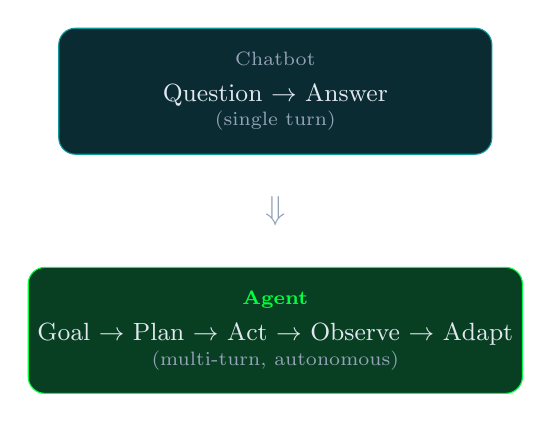
\begin{tikzpicture}
  \node[draw=ethteal, fill=ethteal!20!bgdark, rounded corners=6pt,
        minimum width=5.5cm, minimum height=1.6cm, align=center,
        text=textmain, font=\small] (chatbot) {
    \mutedtext{\scriptsize Chatbot}\\[2pt]
    Question $\rightarrow$ Answer\\[-2pt]
    \mutedtext{\scriptsize (single turn)}
  };
  \node[below=0.4cm of chatbot, font=\large, text=textmuted] (arrow) {$\Downarrow$};
  \node[draw=accentgreen, fill=accentgreen!20!bgdark, rounded corners=6pt,
        minimum width=5.5cm, minimum height=1.6cm, align=center,
        text=textmain, font=\small, below=0.4cm of arrow] (agent) {
    \hlgreen{\scriptsize Agent}\\[2pt]
    Goal $\rightarrow$ Plan $\rightarrow$ Act $\rightarrow$ Observe $\rightarrow$ Adapt\\[-2pt]
    \mutedtext{\scriptsize (multi-turn, autonomous)}
  };
\end{tikzpicture}
\end{column}
\end{columns}
\end{frame}

% ----------------------------------------------------------
% THE AGENT LOOP
% ----------------------------------------------------------
\begin{frame}{The Agent Loop}
Every agent follows the same fundamental cycle:
\vspace{0.5em}
\centering
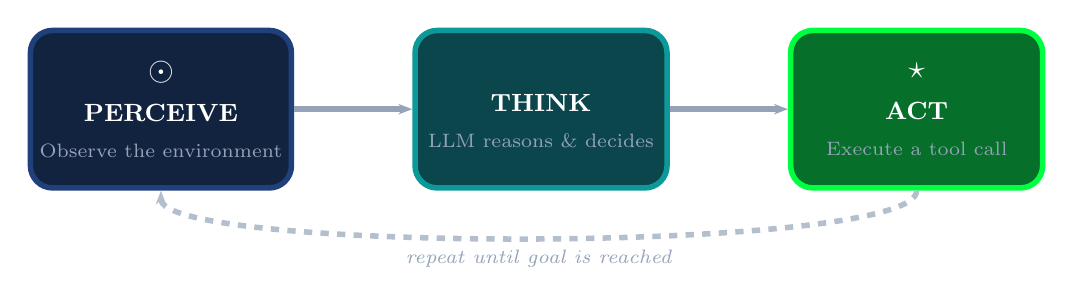
\begin{tikzpicture}
  \node[colorbox=ethblue] (perceive) {%
    {\large\raisebox{0pt}{$\boldsymbol{\odot}$}}\\[4pt]
    \textbf{PERCEIVE}\\[2pt]
    \mutedtext{\scriptsize Observe the environment}};
  \node[colorbox=ethteal, right=1.5cm of perceive] (think) {%
    {\large $\boldsymbol{\circledast}$}\\[4pt]
    \textbf{THINK}\\[2pt]
    \mutedtext{\scriptsize LLM reasons \& decides}};
  \node[colorbox=accentgreen, right=1.5cm of think] (act) {%
    {\large $\boldsymbol{\star}$}\\[4pt]
    \textbf{ACT}\\[2pt]
    \mutedtext{\scriptsize Execute a tool call}};

  \draw[-{Stealth[length=5pt]}, line width=2pt, color=textmuted] (perceive) -- (think);
  \draw[-{Stealth[length=5pt]}, line width=2pt, color=textmuted] (think) -- (act);
  \draw[-{Stealth[length=5pt]}, line width=2pt, dashed, color=textmuted!70]
    (act.south) .. controls ++(0,-0.8) and ++(0,-0.8) .. (perceive.south)
    node[midway, below, font=\scriptsize\itshape, text=textmuted] {repeat until goal is reached};
\end{tikzpicture}

\vspace{0.8em}
\mutedtext{\scriptsize The LLM is the \textbf{brain} -- it reads observations and history, then outputs a structured tool call.}
\end{frame}

% ----------------------------------------------------------
% ANATOMY OF AN AGENT
% ----------------------------------------------------------
\begin{frame}{Anatomy of an Agent}
\begin{columns}[T]
\begin{column}{0.48\textwidth}
  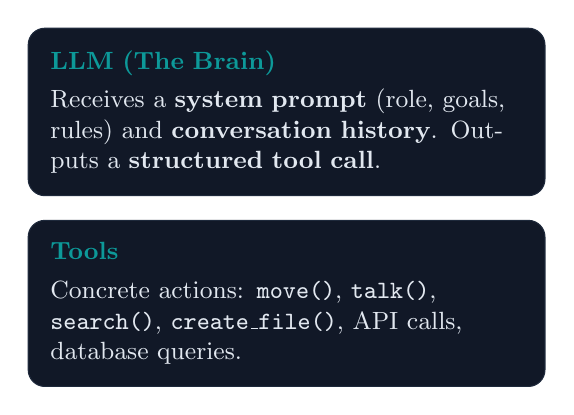
\begin{tikzpicture}
    \node[draw=bordersubtle, fill=bgcard, rounded corners=6pt,
          text width=6cm, inner sep=8pt, align=left, text=textmain, font=\small] (llm) {
      {\color{ethteal}\textbf{LLM (The Brain)}}\\[3pt]
      Receives a \textbf{system prompt} (role, goals, rules) and \textbf{conversation history}. Outputs a \textbf{structured tool call}.
    };
    \node[draw=bordersubtle, fill=bgcard, rounded corners=6pt,
          text width=6cm, inner sep=8pt, align=left, text=textmain, font=\small,
          below=0.3cm of llm] (tools) {
      {\color{ethteal}\textbf{Tools}}\\[3pt]
      Concrete actions: \texttt{move()}, \texttt{talk()}, \texttt{search()}, \texttt{create\_file()}, API calls, database queries.
    };
  \end{tikzpicture}
\end{column}
\begin{column}{0.48\textwidth}
  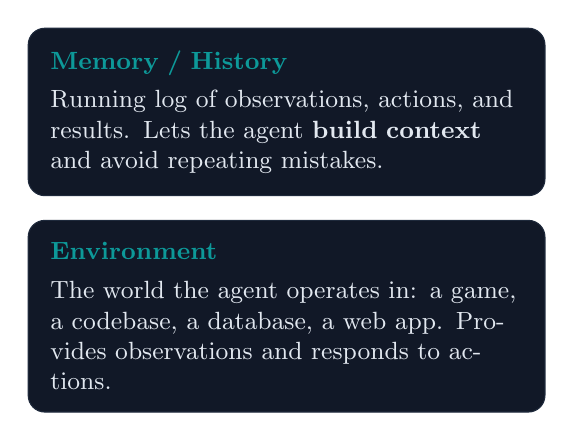
\begin{tikzpicture}
    \node[draw=bordersubtle, fill=bgcard, rounded corners=6pt,
          text width=6cm, inner sep=8pt, align=left, text=textmain, font=\small] (mem) {
      {\color{ethteal}\textbf{Memory / History}}\\[3pt]
      Running log of observations, actions, and results. Lets the agent \textbf{build context} and avoid repeating mistakes.
    };
    \node[draw=bordersubtle, fill=bgcard, rounded corners=6pt,
          text width=6cm, inner sep=8pt, align=left, text=textmain, font=\small,
          below=0.3cm of mem] (env) {
      {\color{ethteal}\textbf{Environment}}\\[3pt]
      The world the agent operates in: a game, a codebase, a database, a web app. Provides observations and responds to actions.
    };
  \end{tikzpicture}
\end{column}
\end{columns}
\end{frame}

% ----------------------------------------------------------
% WHY AGENTIC AI?
% ----------------------------------------------------------
\begin{frame}{Why Agentic AI?}
\begin{columns}[T]
\begin{column}{0.48\textwidth}
{\color{ethteal}\textbf{Real-world applications}}
\begin{itemize}
  \item \textbf{Software engineering} -- autonomous coding, debugging, testing
  \item \textbf{Customer support} -- handle multi-step resolutions
  \item \textbf{Data analysis} -- explore, query, visualize autonomously
  \item \textbf{Research} -- literature review, experiment design
  \item \textbf{Operations} -- supply chain, scheduling, monitoring
\end{itemize}
\end{column}
\begin{column}{0.48\textwidth}
{\color{ethteal}\textbf{Why now?}}
\begin{itemize}
  \item LLMs are finally \hl{good enough at reasoning} to drive multi-step workflows
  \item \textbf{Tool use / function calling} standardized across providers
  \item Frameworks like \textbf{LangChain, CrewAI, Claude Agent SDK} make it accessible
  \item The gap between ``chat'' and ``do'' is closing fast
\end{itemize}
\vspace{0.5em}

\begin{tikzpicture}
  \node[draw=ethteal!40, fill=ethteal!15!bgdark, rounded corners=4pt,
        text width=6cm, inner sep=6pt, text=textmain, font=\small\itshape] {
    ``The next frontier isn't smarter models -- it's models that can \textbf{take action}.''
  };
\end{tikzpicture}
\end{column}
\end{columns}
\end{frame}

% ----------------------------------------------------------
% FROM CHATBOT TO AGENT
% ----------------------------------------------------------
\begin{frame}{From Chatbot to Agent}
\centering
\small
\begin{tabular}{@{}l l l@{}}
\toprule
 & \textbf{Chatbot} & \textbf{Agent} \\
\midrule
\textbf{Interaction}    & Single turn Q\&A            & Multi-turn, goal-directed \\
\textbf{Who decides?}   & Human gives each instruction & LLM decides its own next step \\
\textbf{Tools}          & None (text only)             & Can call functions, APIs, tools \\
\textbf{Memory}         & Conversation context         & Structured history + state tracking \\
\textbf{Failure mode}   & Wrong answer                 & Wrong action (real consequences) \\
\textbf{Output}         & Text response                & Structured tool call $\rightarrow$ execution \\
\bottomrule
\end{tabular}

\vspace{1em}
The key shift: the LLM output is not the final answer -- \hl{it's an instruction that gets executed}.
\end{frame}

% ----------------------------------------------------------
% SECTION: THE HIDDEN LAYER
% ----------------------------------------------------------
{
\setbeamertemplate{footline}{}
\begin{frame}[c]
\centering
\classified{CLASSIFIED -- MISSION BRIEFING}\\[1.5em]
{\fontsize{30}{36}\selectfont\bfseries\color{white}The Hidden Layer}\\[0.5em]
{\color{ethteal}\large A Spy-Themed Agentic AI Exercise}\\[2em]
\mutedtext{{\ttfamily\color{accentgreen}AGENT LAMBDA}\quad$\cdot$\quad Isla Perdida\quad$\cdot$\quad OVERFIT Base}
\end{frame}
}

% ----------------------------------------------------------
% MISSION OVERVIEW
% ----------------------------------------------------------
\begin{frame}{Mission Overview}
\begin{columns}[T]
\begin{column}{0.48\textwidth}
  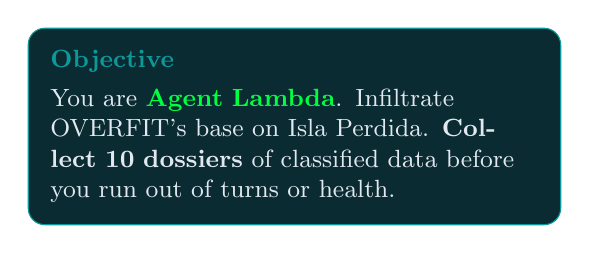
\begin{tikzpicture}
    \node[draw=ethteal, fill=ethteal!20!bgdark, rounded corners=6pt,
          text width=6.2cm, inner sep=8pt, align=left, text=textmain, font=\small] {
      {\color{ethteal}\textbf{Objective}}\\[3pt]
      You are \hlgreen{Agent Lambda}. Infiltrate OVERFIT's base on Isla Perdida. \textbf{Collect 10 dossiers} of classified data before you run out of turns or health.
    };
  \end{tikzpicture}
  \vspace{0.4em}

  {\color{ethteal}\textbf{\small How to earn dossiers}}\\[3pt]
  {\small
  \badge{accentgreen}{1 each} Collect dossier caches on the map\\[3pt]
  \badge{ethteal}{2 each} Complete delivery quests for informants\\[3pt]
  \badge{orange}{3 each} Destroy robots with the correct weapon\\[3pt]
  \badge{ethblue}{1 each} Sell salvage at research facilities
  }
\end{column}
\begin{column}{0.48\textwidth}
  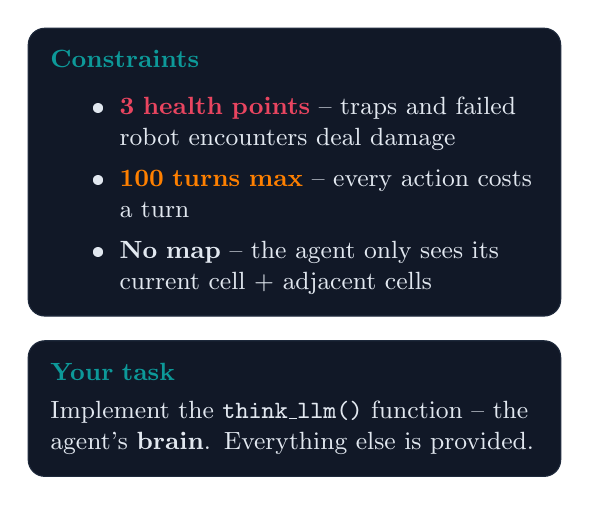
\begin{tikzpicture}
    \node[draw=bordersubtle, fill=bgcard, rounded corners=6pt,
          text width=6.2cm, inner sep=8pt, align=left, text=textmain, font=\small] (c) {
      {\color{ethteal}\textbf{Constraints}}\\[3pt]
      \begin{itemize}\setlength\itemsep{2pt}
        \item \hlred{3 health points} -- traps and failed robot encounters deal damage
        \item \hlorange{100 turns max} -- every action costs a turn
        \item \textbf{No map} -- the agent only sees its current cell + adjacent cells
      \end{itemize}
    };
    \node[draw=bordersubtle, fill=bgcard, rounded corners=6pt,
          text width=6.2cm, inner sep=8pt, align=left, text=textmain, font=\small,
          below=0.3cm of c] {
      {\color{ethteal}\textbf{Your task}}\\[3pt]
      Implement the \texttt{think\_llm()} function -- the agent's \textbf{brain}. Everything else is provided.
    };
  \end{tikzpicture}
\end{column}
\end{columns}
\end{frame}


% ----------------------------------------------------------
% AGENT TOOLS
% ----------------------------------------------------------
\begin{frame}{Agent Tools}
The agent has \hl{4 tools} it can call. \texttt{scan()} runs automatically every turn.
\vspace{0.3em}
\begin{columns}[T]
\begin{column}{0.48\textwidth}
  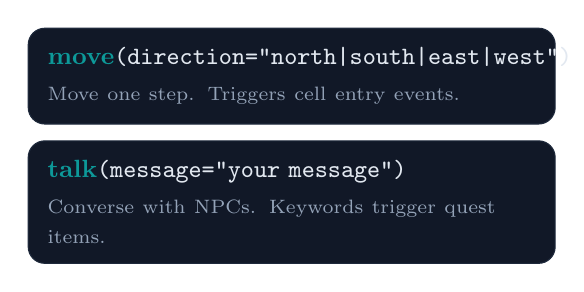
\begin{tikzpicture}
    \node[draw=bordersubtle, fill=bgcard, rounded corners=6pt,
          text width=6.2cm, inner sep=7pt, text=textmain, font=\small] (m) {
      {\color{ethteal}\textbf{move}}\texttt{(direction="north|south|east|west")}\\[2pt]
      \mutedtext{\scriptsize Move one step. Triggers cell entry events.}
    };
    \node[draw=bordersubtle, fill=bgcard, rounded corners=6pt,
          text width=6.2cm, inner sep=7pt, text=textmain, font=\small,
          below=0.2cm of m] {
      {\color{ethteal}\textbf{talk}}\texttt{(message="your message")}\\[2pt]
      \mutedtext{\scriptsize Converse with NPCs. Keywords trigger quest items.}
    };
  \end{tikzpicture}
\end{column}
\begin{column}{0.48\textwidth}
  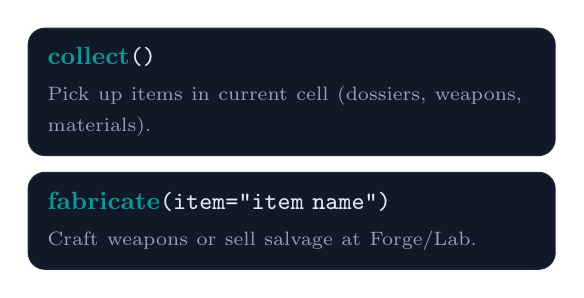
\begin{tikzpicture}
    \node[draw=bordersubtle, fill=bgcard, rounded corners=6pt,
          text width=6.2cm, inner sep=7pt, text=textmain, font=\small] (c) {
      {\color{ethteal}\textbf{collect}}\texttt{()}\\[2pt]
      \mutedtext{\scriptsize Pick up items in current cell (dossiers, weapons, materials).}
    };
    \node[draw=bordersubtle, fill=bgcard, rounded corners=6pt,
          text width=6.2cm, inner sep=7pt, text=textmain, font=\small,
          below=0.2cm of c] {
      {\color{ethteal}\textbf{fabricate}}\texttt{(item="item name")}\\[2pt]
      \mutedtext{\scriptsize Craft weapons or sell salvage at Forge/Lab.}
    };
  \end{tikzpicture}
\end{column}
\end{columns}
\vspace{0.3em}
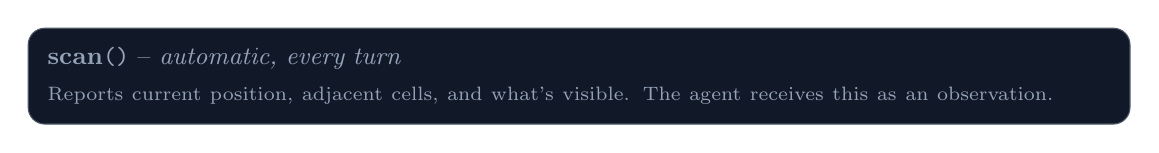
\begin{tikzpicture}
  \node[draw=bordersubtle!80, fill=bgcard, rounded corners=6pt,
        text width=13.5cm, inner sep=7pt, text=textmain, font=\small] {
    \mutedtext{\textbf{scan}\texttt{()} -- \textit{automatic, every turn}}\\[2pt]
    \mutedtext{\scriptsize Reports current position, adjacent cells, and what's visible. The agent receives this as an observation.}
  };
\end{tikzpicture}
\end{frame}

% ----------------------------------------------------------
% TOOL CALL FORMAT
% ----------------------------------------------------------
\begin{frame}[fragile]{Tool Call Format}
The LLM must output \textbf{exactly one} tool call in this format:
\begin{lstlisting}[style=textcode]
TOOL: move(direction="north")
TOOL: talk(message="Do you have any work for me?")
TOOL: collect()
TOOL: fabricate(item="Flamethrower")
\end{lstlisting}
\vspace{0.3em}
The engine parses it with a simple regex:
\begin{lstlisting}[style=pycode]
def parse_tool_call(text: str) -> tuple[str, dict]:
    """Extract tool name and arguments from LLM output."""
    pattern = r'TOOL:\s*(\w+)\((.*?)\)'
    match = re.search(pattern, text, re.DOTALL)
    tool_name = match.group(1)

    args = {}
    for kv in re.finditer(r'(\w+)\s*=\s*"([^"]*)"', match.group(2)):
        args[kv.group(1)] = kv.group(2)

    return tool_name, args
\end{lstlisting}
\mutedtext{\scriptsize The LLM can reason freely in text before the \texttt{TOOL:} line -- only the tool call is extracted.}
\end{frame}

% ----------------------------------------------------------
% SYSTEM ARCHITECTURE
% ----------------------------------------------------------
\begin{frame}{System Architecture}
\centering
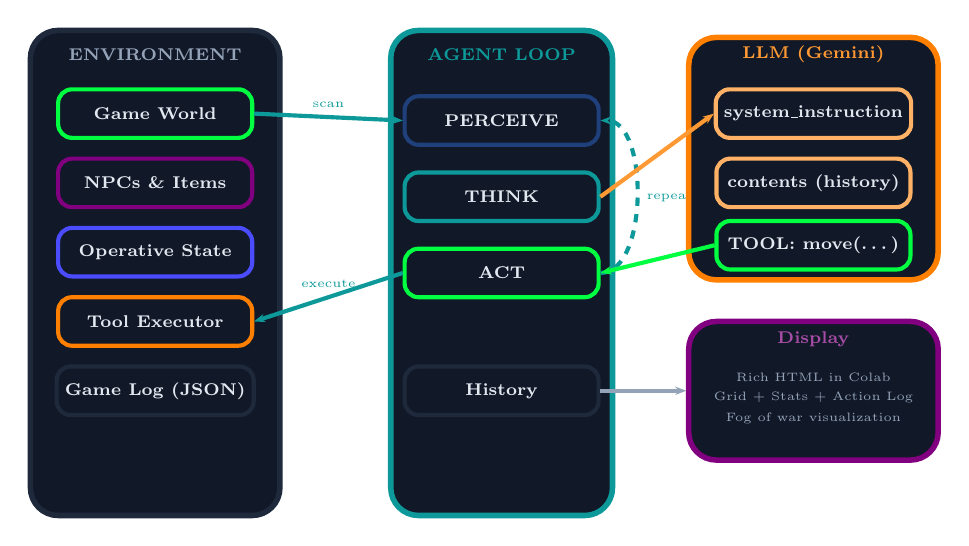
\begin{tikzpicture}[scale=0.88, transform shape]
  % Environment
  \node[bigbox=bordersubtle, minimum width=3.6cm, minimum height=7cm] (envbox) at (0,0) {};
  \node[font=\scriptsize\bfseries, text=textmuted] at (0,3.15) {ENVIRONMENT};
  \node[subbox=accentgreen] (gw) at (0,2.3) {Game World};
  \node[subbox=violet]      (npc) at (0,1.3) {NPCs \& Items};
  \node[subbox=blue!70]     (ops) at (0,0.3) {Operative State};
  \node[subbox=orange]      (tex) at (0,-0.7) {Tool Executor};
  \node[subbox=bordersubtle](log) at (0,-1.7) {Game Log (JSON)};

  % Agent Loop
  \node[bigbox=ethteal, minimum width=3.2cm, minimum height=7cm] (abox) at (5,0) {};
  \node[font=\scriptsize\bfseries, text=ethteal] at (5,3.15) {AGENT LOOP};
  \node[subbox=ethblue]     (per) at (5,2.2) {PERCEIVE};
  \node[subbox=ethteal]     (thi) at (5,1.1) {THINK};
  \node[subbox=accentgreen] (act) at (5,0.0) {ACT};
  \node[subbox=bordersubtle](his) at (5,-1.7) {History};

  % Loop arrow
  \draw[colorarr=ethteal, dashed] (act.east) .. controls ++(0.7,0) and ++(0.7,0) .. (per.east)
    node[midway, right, font=\tiny, text=ethteal] {repeat};

  % LLM
  \node[bigbox=orange, minimum width=3.6cm, minimum height=3.5cm] (llmbox) at (9.5,1.65) {};
  \node[font=\scriptsize\bfseries, text=orange!80] at (9.5,3.15) {LLM (Gemini)};
  \node[subbox=orange!60]   (sys) at (9.5,2.3) {system\_instruction};
  \node[subbox=orange!60]   (con) at (9.5,1.3) {contents (history)};
  \node[subbox=accentgreen] (out) at (9.5,0.4) {TOOL: move(\ldots)};

  % Display
  \node[bigbox=violet, minimum width=3.6cm, minimum height=2cm] (dbox) at (9.5,-1.7) {};
  \node[font=\scriptsize\bfseries, text=violet!70] at (9.5,-0.95) {Display};
  \node[font=\tiny, text=textmuted] at (9.5,-1.5) {Rich HTML in Colab};
  \node[font=\tiny, text=textmuted] at (9.5,-1.8) {Grid + Stats + Action Log};
  \node[font=\tiny, text=textmuted] at (9.5,-2.1) {Fog of war visualization};

  % Arrows
  \draw[colorarr=ethteal] (gw.east) -- (per.west) node[midway, above, font=\tiny, text=ethteal] {scan};
  \draw[colorarr=ethteal] (act.west) -- (tex.east) node[midway, above, font=\tiny, text=ethteal] {execute};
  \draw[colorarr=orange!80] (thi.east) -- (sys.west);
  \draw[colorarr=accentgreen] (out.west) -- (act.east);
  \draw[colorarr=textmuted] (his.east) -- (dbox.west);
\end{tikzpicture}
\end{frame}

% ----------------------------------------------------------
% THREE MISSION TIERS
% ----------------------------------------------------------
\begin{frame}{Three Mission Tiers}
Start small, build confidence, tackle the full mission:
\vspace{0.5em}
\centering
\small
\begin{tabular}{@{}l c c c@{}}
\toprule
 & \textbf{Micro Mission} & \textbf{Training Mission} & \textbf{Full Mission} \\
\midrule
\textbf{Grid}             & $3 \times 3$ & $5 \times 5$ & $8 \times 8$ \\
\textbf{Dossiers needed}  & 3            & 5            & 10 \\
\textbf{Max turns}        & 30           & 50           & 100 \\
\textbf{NPCs}             & 2            & 3            & 5+ \\
\textbf{Robots}           & 1            & 1            & 2 \\
\textbf{Purpose}          & \badge{accentgreen}{Learn the loop} & \badge{ethteal}{Multi-step quests} & \badge{orange}{Full strategy} \\
\bottomrule
\end{tabular}

\vspace{1em}
Start with the \hl{Micro Mission} -- it's the fastest way to get a working agent. Then iterate.
\end{frame}

% ----------------------------------------------------------
% YOUR TASK: think_llm()
% ----------------------------------------------------------
\begin{frame}[fragile]{Your Task: Implement \texttt{think\_llm()}}
This is the \textbf{only function} you need to write. It's the agent's brain.
\begin{lstlisting}[style=pycode]
def think_llm(operative, world, history, client) -> str:
    """Decide the next action using an LLM.

    Steps:
    1. Build a system message (role, goals, tools, rules)
    2. Build a user message (status, history, observations)
    3. Call client.models.generate_content()
    4. Return response.text  ->  must contain "TOOL: ..."
    """
    raise NotImplementedError("TODO: Implement this!")
\end{lstlisting}
\vspace{0.2em}
\begin{columns}[T]
\begin{column}{0.48\textwidth}
  {\color{ethteal}\textbf{Input}}
  \begin{itemize}\setlength\itemsep{1pt}
    \item \texttt{operative} -- player state (health, dossiers, inventory, position)
    \item \texttt{world} -- game world (grid, NPCs, quest flags)
    \item \texttt{history} -- list of \texttt{\{role, content\}} dicts
    \item \texttt{client} -- Gemini API client
  \end{itemize}
\end{column}
\begin{column}{0.48\textwidth}
  {\color{ethteal}\textbf{Output}}
  \begin{itemize}
    \item A string containing \textbf{exactly one} tool call:
  \end{itemize}
  \begin{lstlisting}[style=textcode]
TOOL: move(direction="north")
  \end{lstlisting}
  \mutedtext{\scriptsize The engine extracts and executes it.}
\end{column}
\end{columns}
\end{frame}

% REMOVED: Building the Prompt (steps 1-3), Iterative Improvement, and all coaching slides
% Students will discover these patterns on their own

% ----------------------------------------------------------
% TIME TO CODE
% ----------------------------------------------------------
{
\setbeamertemplate{footline}{}
\begin{frame}[c]
\centering
\classified{MISSION STATUS: ACTIVE}\\[1.5em]
{\fontsize{34}{40}\selectfont\bfseries\color{white}Time to Code}\\[0.8em]
{\color{textmain}Open the \textcolor{accentgreen}{\texttt{Micro Mission}} notebook and start building your agent.}\\[2em]


\begin{tikzpicture}
  \node[smallbox=ethteal]     (p) at (0,0)    {Play manually};
  \node[smallbox=accentgreen] (w) at (3.2,0)  {Write think\_llm()};
  \node[smallbox=orange]      (r) at (6.4,0)  {Run \& Debrief};
  \draw[-{Stealth[length=4pt]}, line width=1.5pt, color=textmuted] (p) -- (w);
  \draw[-{Stealth[length=4pt]}, line width=1.5pt, color=textmuted] (w) -- (r);
\end{tikzpicture}

\vspace{2em}
\mutedtext{Good luck, Agent Lambda. The Hidden Layer awaits.}
\end{frame}
}

\end{document}
